\documentclass[12pt,a4paper,oneside]{book}


% \newcommand{\project}{III}
\newcommand{\projectname}{
	Học tăng cường\par
}
% \newcommand{\specialized}{Toán Tin}
% \newcommand{\orientation}{Tin học}
% \newcommand{\studentname}{Phùng Trọng Hiếu}
\newcommand{\teachername}{TS. Nguyễn Thị Ngọc Anh}
% \newcommand{\studentclass}{Toán Tin 01-K60}
% \newcommand{\studentcode}{20151366}


\usepackage[utf8]{inputenc}
\usepackage[utf8]{vietnam}
\usepackage{amsmath} % Required to use mathematical features
\usepackage{amsfonts}
\usepackage{amssymb}
\usepackage{float} % Fixed positions of figures
\usepackage{gensymb}
\usepackage{geometry}
\geometry{
	a4paper,
	tmargin=35mm,
	bmargin=30mm,
	lmargin=35mm,
	rmargin=20mm,
}
\usepackage{mathptmx} % the replacement of Times New Roman
\linespread{1.25} % same as 1.5 line spacing in MS Word
\usepackage{graphicx}
\graphicspath{{images/}}
\usepackage{enumerate}
\usepackage{indentfirst}
\usepackage{fancybox}
\usepackage{fancyhdr}

\pagestyle{fancy}
\fancyhf{}
\lhead{\textit{\chaptername\space\thechapter}}
\rhead{\textit{GVHD: \teachername}}
% \lfoot{\textit{SVTH: \studentname}}
% \rfoot{\textit{\studentclass}}
\cfoot{\textit{\thepage}}
\fancyfoot[C]{\textit{\thepage}}
\renewcommand{\headrulewidth}{1pt}
\renewcommand{\footrulewidth}{1pt}

\fancypagestyle{plain}{
	\fancyhf{} % clear all header and footer fields
	\fancyfoot[C]{\textit{\thepage}} % except the center
	\renewcommand{\headrulewidth}{0pt}
	\renewcommand{\footrulewidth}{0pt}
}

\newtheorem{theorem}{Định lý}[section]
\newtheorem{lemma}[theorem]{Lemma}
\newtheorem{corollary}[theorem]{Hệ quả}
\newtheorem{cy}[theorem]{Chú ý} 
% \newtheorem{definition}[theorem]{Định nghĩa}%[section]
\newtheorem{bd}[theorem]{Bổ đề} 
\newtheorem{bt}[theorem]{Bài toán}
\newtheorem{md}[theorem]{Mệnh đề} 
\newtheorem{remark}[theorem]{Nhận xét} 
\newtheorem{Bt}[theorem]{Bài toán} 
\newtheorem{example}[theorem]{Ví dụ} 
\newtheorem{hq}[theorem]{Hệ quả}
\newtheorem{kh}[theorem]{Kí hiệu}
\newtheorem{cor}[theorem]{Hệ quả}
\newtheorem{dfn}[theorem]{Định nghĩa}%[section]
\newtheorem{lem}[theorem]{Bổ đề} 
\newtheorem{prop}[theorem]{Mệnh đề} 
\newtheorem{dl}[theorem]{Định lý}
\newtheorem{vd}[theorem]{\bf Ví dụ} 
\newtheorem{nx}[theorem]{ Nhận xét} 
\newtheorem{dn}[theorem]{\bf Định nghĩa} 
\newtheorem{tc}[theorem]{\bf Tính chất} 
\newtheorem{ch}[theorem]{\bf Câu hỏi} 
\newtheorem{ttt}[theorem]{\bf Thuật toán} 
\newtheorem{gt}[theorem]{\bf Giả thiết} 

\usepackage[backend=bibtex,style=ieee, sorting=nty]{biblatex}
\addbibresource{project_ref.bib}


\begin{document}
\begin{titlepage}
	\thisfancypage{\setlength{\fboxsep}{10pt}\doublebox}{}
	\begin{center}
		\begin{Large}\bfseries
			TRƯỜNG ĐẠI HỌC BÁCH KHOA HÀ NỘI\par
			VIỆN TOÁN ỨNG DỤNG VÀ TIN HỌC\par
		\end{Large}
		\vspace{1.5cm}
		
\includegraphics[scale=0.3]{images/logo_bk.jpg}\par
		\vspace{1.5cm}
		\begin{LARGE}
			\MakeUppercase{Báo cáo môn học}\par
		\end{LARGE}
		\begin{LARGE}
			\MakeUppercase{Các mô hình ngẫu nhiên và ứng dụng}\par
		\end{LARGE}
		\vspace{1.5cm}
		\begin{Large}
			\MakeUppercase{Đề tài: \projectname}
		\end{Large}
		\vspace{1cm}
		\begin{large}
			% ĐỒ ÁN \project\par
			% \vspace{0.5cm}
			% Chuyên ngành: \MakeUppercase{\specialized}\par
			% \vspace{0.5cm}
			% Chuyên sâu: \orientation\par
			\begin{flushleft}
				\hspace{2cm}
				Giảng viên hướng dẫn: \MakeUppercase{\textbf{\teachername}}\par
				\vspace{0.5cm}
				\hspace{2cm}
				Nhóm sinh viên thực hiện:\par
				% \textbf{PHÙNG TRỌNG HIẾU}\par
				% \hspace{2cm}
				
				% \textbf{CAO ĐĂNG SAO}\par
				% \hspace{2cm}
				% 				\textbf{NINH NGỌC LUYÊN}\par
				% \hspace{2cm}
				
				% \textbf{NGUYỄN MẠNH CƯỜNG}\par
				\begin{table}[H]
					\hspace{4.5cm}
					\begin{tabular}{ll}
					\textbf{PHÙNG TRỌNG HIẾU}  & \textbf{20151366} \\
					\textbf{CAO ĐĂNG SAO}      & \textbf{20163476} \\
					\textbf{NINH NGỌC LUYÊN}   & \textbf{20142747} \\
					\textbf{NGUYỄN MẠNH CƯỜNG} & \textbf{20140596}
					\end{tabular}
				\end{table}

				% \hspace{2.5cm}
				% Sinh viên thực hiện: \MakeUppercase{\studentname}\par
				% \hspace{2.5cm}
				% Lớp: \studentclass\par
				% \hspace{2.5cm}
				% MSSV: \studentcode\par
			\end{flushleft}
		\end{large}
		\vfill
		\begin{large}\bfseries
			HÀ NỘI - \the\year\par
		\end{large}
	\end{center}
\end{titlepage}

\frontmatter

% \chapter*{\centering\LARGE\MakeUppercase{Nhận xét của giảng viên hướng dẫn}}
% \begin{enumerate}
% 	\item Mục đích và nội dung của đồ án:\par
% 	\dotfill\par\dotfill\par\dotfill\par\dotfill\par\dotfill
% 	\item Kết quả đạt được:\par
% 	\dotfill\par\dotfill\par\dotfill\par\dotfill\par\dotfill
% 	\item Ý thức làm việc của sinh viên:\par
% 	\dotfill\par\dotfill\par\dotfill\par\dotfill\par\dotfill
% \end{enumerate}
% \hfill
% \begin{minipage}[t]{0.48\textwidth}
% 	\begin{center}
% 		Hà Nội, ngày\hspace{5mm}tháng\hspace{5mm}năm\par
% 		Giảng viên hướng dẫn\par
% 		\textit{(Ký và ghi rõ họ tên)}
% 	\end{center}
% \end{minipage}

\renewcommand{\listfigurename}{Danh mục hình vẽ}
\listoffigures
% \listoftables

\chapter{Lời cảm ơn}
Để hoàn thành được báo cáo môn học: "Các mô hình ngẫu nhiên và ứng dụng",
lời đầu tiên chúng em xin chân thành cảm ơn cô giáo hướng dẫn \teachername\space
đã truyền đạt những kinh nghiệm, kỹ năng, kiến thức nền tảng
để giúp chúng em hoàn thành báo cáo môn học này.

% Em cũng xin chân thành cảm ơn thầy giáo Lê Chí Ngọc đã cho em nhiều lời khuyên quý báu
% cùng các thầy cô trong viện Toán ứng dụng và Tin học Trường Đại học Bách Khoa Hà Nội
% đã truyền đạt những kinh nghiệm, kỹ năng, kiến thức nền tảng để giúp em hoàn thành đồ án môn học này.

% Xin cảm ơn các anh, các chị của phòng Machine Learning tại Công Ty TNHH Công Nghệ Cao SkymapGlobal Việt Nam
% đã hỗ trợ em về trang thiết bị và công nghệ.

Cảm ơn tất cả các bạn trong lớp
đã cho nhóm mình những ý kiến đóng góp và giúp đỡ trong quá trình làm báo cáo.

Tuy đã có những cố gắng nhất định, tìm hiểu và tiếp cận với đề tài
nhưng do trình độ và thời gian hạn chế
nên báo cáo này không thể tránh khỏi các thiếu sót.
Rất mong nhận được những nhận xét góp ý và sửa sai của cô giáo hướng dẫn,
các thầy cô, và các bạn để quyển báo cáo này trở nên hoàn thiện hơn.

Nhóm chúng em xin chân thành cảm ơn!

\hfill
\begin{minipage}[t]{0.48\textwidth}
	\begin{center}
		Hà Nội, ngày \the\day\space tháng \the\month\space năm \the\year\par
		Trưởng nhóm\par
		Phùng Trọng Hiếu
	\end{center}
\end{minipage}

\tableofcontents

\mainmatter

\chapter{Giới thiệu}
\label{ch:intro}



\chapter{Quá trình Markov}
\label{ch:02}
	Chương này trình bày định nghĩa, một số ví dụ về Xích Markov và Quá trình Markov. Kiến thức của chương được tổng hợp từ tài liệu \cite{Gagniuc2017}.
\section{Xích markov}
\begin{dn} \rm
Cho không gian trạng thái $E$,$\lbrace S_{t}\rbrace _{t\geq 0}$ được gọi là một xích Markov nếu nó thỏa mãn tính không nhớ:
\begin{align}
P(S_{t+1}=s_{t+1}|S_{t}=s_{t},S_{t-1}=s_{t-1},...,S_{0}=s_{0}) = P(S_{t+1}=s_{t+1}|S_{t}=s_{t}),
\end{align}
với $t\in \mathbb{N}$ và $s_{i} \in E, i = 0,1,...,t+1.$
\end{dn}

\begin{vd}
Xích Markov các trạng thái của một sinh viên trong lớp với xác suất chuyển được minh họa như Hình 2.1. 
\begin{itemize}
\item Tập không gian trạng thái $S = \lbrace FB,C,Pt,Sl \rbrace $ tương ứng với các hoạt động Facebook, Class, Party và Sleep của sinh viên.
\item Ma trận xác suất chuyển:
\begin{align*}
\begin{bmatrix}
0.9&  0.1&  0& 0\\ 
0.5&  0&  0.4& 0.1\\ 
0&  0.5& 0 & 0.5\\ 
0 & 0 & 0 & 1
\end{bmatrix}
\end{align*}
\end{itemize}
\newpage
\begin{figure}[ht] {\label{h2.1}}
    \centering
    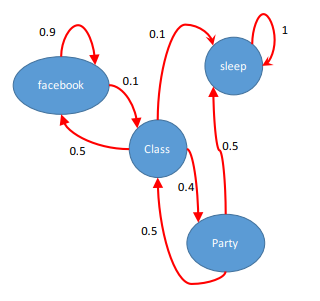
\includegraphics[scale=0.7]{vidumarkovchain.png}
    \caption{Sơ đồ chuyển trạng thái của sinh viên.}
    \label{fig:tactumoitruong}
\end{figure}
\end{vd}
\section{Quá trình Markov}
\begin{dn} \rm
$\lbrace S_{t}\rbrace _{t\geq 0}$ với không gian trạng thái hữu hạn $E$ được gọi là quá trình Markov nếu thỏa mãn :
\begin{align}
P(S_{t+s}=j|S_{u};u\leq t)=P(S_{t+s}=j|S_{t}).
\end{align}
\end{dn}
\begin{nx} \rm
Nếu $Pr(S_{t+s}=j|S_{t}=i)=Pr(S_{s}=j|S_{0}=j)$ thì quá trình Markov này được gọi là quá trình Markov dừng.
\end{nx}

\chapter{Chương 3}
\label{ch:03}



\chapter{Thuật toán Q-Learning và Deep Q-Learning}
\label{ch:04}
\section{Q-Learning}
\subsection{Giới thiệu}
Những thuật toán học tăng cường thông thường gồm có quy hoạch động (Dynamic
Programming), Monte-Carlo và phương pháp TD (Temporal-Difference). Tuy nhiên các phương
pháp quy hoạch động và Monte-Carlo không hiệu quả do đòi hỏi bộ nhớ quá lớn, hoặc mô hình
phải xác định hay khó hội tụ nên ít khi cho ra kết quả tối ưu. Phương pháp TD là sự kết hợp của
hai phương pháp quy hoạch động, Monte-Carlo và nó còn cho phép giải quyết được nhiều bài toán thực tế bởi vì phương
pháp này không đòi hỏi môi trường xác định và có khả năng hội tụ cao. Một biến thể của
phương pháp TD được gọi là Q-learning. Nó là một phương pháp học kiểu TD theo hướng off-policy,
rất hiệu quả trong việc giải quyết các bài toán tìm đường. Quá trình học tăng cường có thể được thực
hiện theo hai cách: off-policy và on-policy. On-policy sử dụng một chiến lược chọn hành động để thực
hiện các bước hành động để tối ưu hóa chính chiến lược chọn hành động đó. Phương pháp off-policy
sử dụng một chiến lược chọn hành động để thực hiện các hành động nhưng với mục đích là để tối ưu
hóa một chiến lược chọn hành động khác.
\subsection{Thuật toán Q-Learning}
Cho một chiến lược (policy) $\pi$, ta viết lại công thức (trình bày ở chương 3) về Q-value (hay là giá trị hành động)
như sau:
\begin{equation} 
    \label{eq:Qvalue}
    Q^{\pi}(s,a) = R(s,a) + \gamma \sum_{s'\in \S} P_{ss^{'}}^{a}V^{\pi}(s').
\end{equation}
Trong công thức \ref{eq:Qvalue}, $Q^{\pi}(s,a)$ là Q-value khi thực hiện hành động a tại trạng thái s theo chiến lược $\pi$; $R(s,a)$ là phần thưởng nhận được; $s^{'}$ là trạng thái kế tiếp. $\gamma$ là hệ số giảm (discount rate), đảm bảo "gần" đích Q-value càng lớn.\\
Nói các khác, Q-value là hàm giá trị hành động mong đợi cho việc thực hiện hành động $a$ ở trạng thái $s$ và tuân theo chính sách $\pi$ sau đó. 
 Mục đích của Q-learning là ước lượng Q-values cho một chiến lược tối ưu. Để tiện lợi, ta định nghĩa như sau 
 $Q^{*}(s,a) \equiv Q^{\pi^{*}}(s,a), \forall s, a$. Thật đơn giản để chỉ ra rằng
  $V^{*}(s) = max_{a} Q^{*}(s,a)$ và nếu $a^{*}$ là một hành động mà tại đó
  mức tối đa đạt được, sau đó một chiến lược tối ưu có thể được hình thành như $\pi^{*}(s) \equiv a^{*}$.
  Ở đây, lợi ích của những giá trị Q-value là nếu một tác tử (agent) có thể học chúng, nó có thể 
  dễ dàng quyết định đâu là tối ưu để hành động. Mặc dù có thể có nhiều hơn một chiến lược tối ưu hay 
  $a^{*}$, những giá trị $Q^{*}$ là duy nhất.\\
  \indent Trong Q-learning,  kinh nghiệm của tác tử (agent) bao gồm một chuỗi tuần tự các quá trình riêng biệt (gọi là Episodes).\\
  Trong episode thứ n, tác tử sẽ:
\begin{itemize}
    \item quan sát trạng thái hiện tại của nó $s_n$,
    \item lựa chọn và thực hiện một hành động $a_n$,
    \item quan sát trạng thái tiếp theo $s_{n+1}$,
    \item nhận được ngay phần thưởng $r_n$, và
    \item điều chỉnh các giá trị $Q_{n-1}$ của nó bằng cách sử dụng hệ số học $\alpha_{n}$, theo:
\end{itemize}
\begin{equation} 
Q_{n}(s,a) =  \begin{cases}
    (1-\alpha_n)Q_{n-1}(s,a) + \alpha_{n}[r_n + \gamma V_{n-1}(s_{n+1})] &\text{nếu } s = s_n \text{ và } a = a_n,\\
    Q_{n-1}(s, a) &\text{trường hợp khác}
\end{cases}   
\end{equation}
Trong đó :
\begin{equation} 
    \label{eq:Vn}
    V_{n-1}(s) \equiv max_{b} {Q_{n-1}(s,b)}
\end{equation}
là tốt nhất mà tác tử có thể làm được từ trạng thái s. Dĩ nhiên, ở những giai đoạn đầu việc học thì Q-value có thể không phản ánh 
đúng chiến lược mà chúng đã được biết (việc tối đa hóa các hành động ở phương trình \ref{eq:Vn}). 
Hiển nhiên là các giá trị Q-value ban đầu, $Q_{0}(s,a)$, cho tất cả các trạng thái và hành động đã được giả thiết. Ngoài ra ta có thêm 
giải thiết một bảng tra cứu (look-up table) biểu diễn cho $Q_n(s,a)$. 
Theo ~\cite{Watkins1989} cho thấy Q-learning có thể không hội tụ chính xác cho các biểu diễn khác.\\
\indent Phân tích thuật toán Q-learning, ta có các bước như sau:
\begin{itemize}
    \item 1. Khởi tạo bảng Q với các số 0 và giá trị Q thành các hằng số tùy ý.
    \item 2. Khám phá các hành động: đối với mỗi thay đổi về trạng thái, chọn bất 
    kỳ một hành động (a) nào trong số tất cả các hành động có thể có cho trạng thái 
    hiện tại (S).
    \item 3. Đi đến trạng thái tiếp theo (S') là kết quả của hành động (a).
    \item 4. Đối với tất cả các hành động có thể từ trạng thái (S,), hãy chọn một hành 
    động có giá trị Q cao nhất.
    \item 5. Cập nhật giá trị bảng Q bằng phương trình.
    \item 6. Đặt trạng thái tiếp theo làm trạng thái hiện tại.
    \item 7. Nếu trạng thái cuối đạt được, sau đó kết thúc và lặp lại quá trình.
\end{itemize}
\subsection{Sự hội tụ của thuật toán}
Điều kiện quan trọng nhất trong định lý hội tụ được đưa ra dưới đây là chuỗi các quá trình (Episodes) hình thành nền tảng học tập phải 
bao gồm vô hạn quá trình cho mỗi trạng thái và hành động bắt đầu. Đây có thể được coi là một điều kiện mạnh về cách lựa chọn các 
trạng thái và hành động, tuy nhiên, trong các điều kiện ngẫu nhiên của định lý, không có phương pháp nào có thể được đảm bảo 
để tìm ra một chiến lược tối ưu trong các điều kiện yếu hơn. Tuy nhiên, xin lưu ý rằng các quá trình không cần phải tạo thành một 
chuỗi liên tục, đó là $y$ của một quá trình không cần phải là $x$ của quá trình tiếp theo.\\
\indent Định lý dưới đây định nghĩa một tập các điều kiện theo đó $Q_n(s,a) \to Q^{*}(s,a)$ khi $n \to \infty$. 
Định nghĩa $n^{i}(s, a)$ là chỉ số của lần thứ i mà hành động a được thử ở trạng thái s.
Định lý hội tụ thuật toán Q-learning:
\begin{theorem}
    \label{th:Conver}
    Cho một miền phần thưởng bị chặn $r_n \leq R$, tỉ lệ học $0 \leq \alpha_n < 1$, và
    \begin{equation}
        \sum_{i=1}^{\infty}\alpha_{n^{i}(s,a)} = \infty, \sum_{i=1}^{\infty}[\alpha_{n^{i}(s,a)}]^2 < \infty, \forall s, a,
    \end{equation} 
    thì $Q_n(s,a) \to Q^{*}(s,a)$ khi $n \to \infty, \forall x, a,$ với xác suất bằng 1.
\end{theorem}
Chứng minh tính đúng đắn của định lý \ref{th:Conver} xem chi tiết trong~\cite{Watkins1992}.
\section{Deep Q-Learning}
Mục đích của bài toán là chọn ra hành động (action) thích hợp cho một trạng thái nào đó (state) 
nào đó. Hay nói cách khác, với state là đầu vào và cần đầu ra là một hành động. 
Công việc đó sẽ được thực hiện qua một mang nơ-ron (Neural Network-NN). Những gì ta cần làm 
chỉ là bỏ đi  bảng tra cứu lookup table $Q(s,a)$ và thay thế bằng một mạng nơ-ron đơn giản. 
Điều đó được mô tả trong Hình \ref{fig:qlearning}.
\begin{figure}[ht]
    \centering
    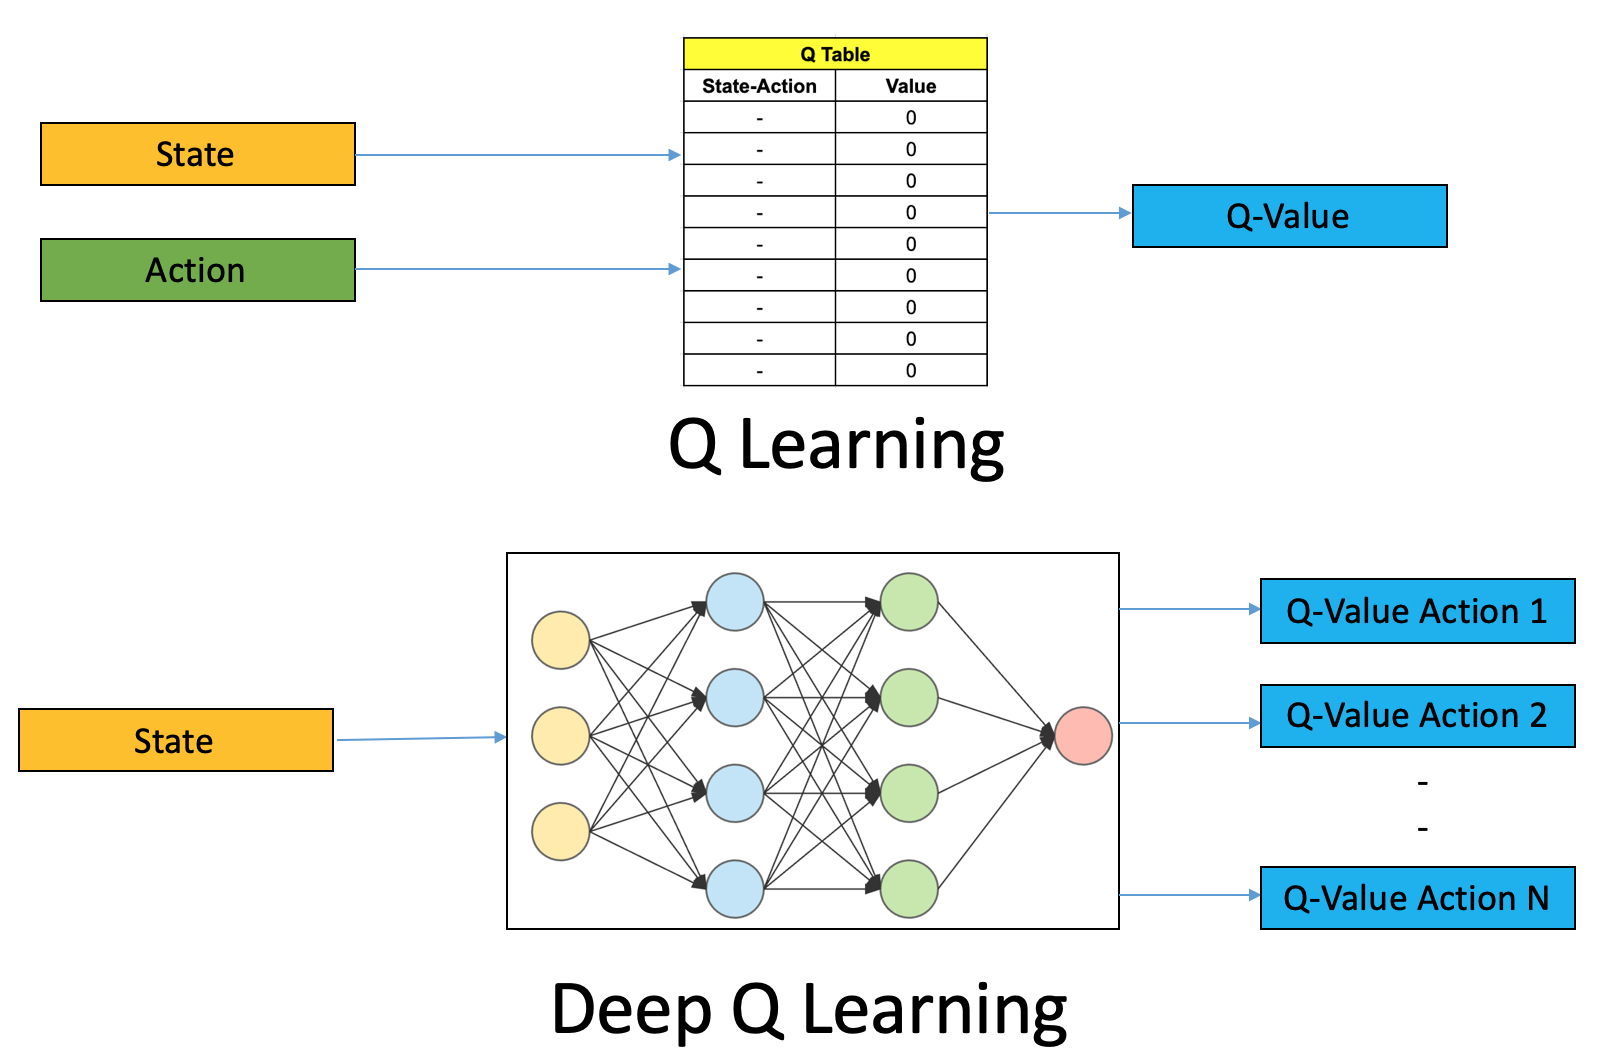
\includegraphics[width=\textwidth]{qvsdeepQlearning.png}
    \caption{So sánh về cấu trúc giữa Q-learning và Deep Q-learning.}
    \label{fig:qlearning}
\end{figure}
\subsubsection{Hàm mất mát}
Mục đích của ta là bắt mạng học được cách ước lượng Q-Value cho các hành động một cách chính xác nên đương nhiên 
hàm mất mát phải tính được sai số giữa Q-value thực tế và dự đoán. Hàm mất mát định nghĩa dưới dạng đầy đủ 
như sau:
\begin{equation}
    \label{eq:lossf}
    Loss = (r + \gamma max_{a'}Q(s', a'; \theta') - Q(s, a; \theta))^2
\end{equation}
\subsubsection{Kinh nghiệm chơi lại (Experience replay)} 
Ở phần trên ta đã định nghĩa một mạng nơ-ron lấy input là state hiện tại và output các Q-value. 
Thế nhưng nếu mạng nơ-ron  cứ liên tục bị đẩy vào từng state một sẽ rất dễ bị overfitting 
vì các states liên tục thường giống nhau hoặc có tính tuyến tính (ví dụ: liên tục 
đi thẳng/sang trái/phải). Kỹ thuật Experience Replay được sử dụng để loại bỏ vấn đề này.
 Thay vì mỗi state mạng update một lần, ta lưu lại các states vào bộ nhớ (memory).
 Sau đó thực hiện sampling thành các batch nhỏ đưa vào mạng nơ-ron học. Việc này giúp đa 
 dạng hóa input và tránh mạng nơ-ron bị overfitting.
 \subsubsection{Mô hình}
 Mô hình đầy đủ của Deep Q-Learning được mô tả trong Hình \ref{fig:deepqlearning}
 \begin{figure}[ht]
    \centering
    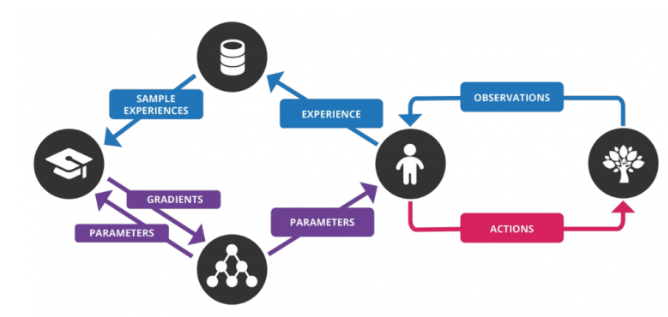
\includegraphics[width=\textwidth]{model.png}
    \caption{Mô hình Deep Q-Learning.}
    \label{fig:deepqlearning}
\end{figure}
\subsubsection{\underline{Tóm lại}}
Deep Q-Learning thực hiện các bước sau:
\begin{itemize}
    \item 1. Enviroment đưa vào mạng một state s; đầu ra là các Q-value của các actions tương ứng.
    \item 2. Agent chọn action bằng một Policy và thực hiện action a đó.
    \item 3. Environment trả lại state s' cùng với reward r tương ứng và lưu lại experience s, a, r, s'.
    \item 4. Thực hiện sample các experience thành một vài batches và tiến hành luyện mạng.
    \item 5. Lặp lại đến khi kết thúc M episodes.
\end{itemize}

\chapter{Một số bài toán ứng dụng}
\label{ch:05}

Trong chương này, ta sẽ cùng nhau giải quyết
hai bài toán học tăng cường cơ bản để minh họa cho việc
sử dụng thuật toán Q-Learning đã được trình bày ở chương trước.
Bài toán đầu tiên sẽ là bài Chiếc taxi thông minh (Smart Taxi);
trong bài toán này, ta sẽ huấn luyện một chiếc taxi
sao cho nó có thể đón và trả khách tại đúng vị trí
và thực hiện việc này một cách "thông minh" nhất có thể.
Bài toán thứ hai sẽ giải quyết việc điều khiển
chiếc xe đẩy để giữ cho con lắc được gắn trên xe
luôn ở trạng thái cân bằng; bài toán kinh điển này còn
được biết đến với cái tên Bài toán cân bằng con lắc ngược (CartPole).

\section{Bài toán chiếc taxi thông minh}
\subsection{Bài toán}
Ta có một chiếc taxi được trang bị các cảm biến, trí tuệ nhân tạo,~\dots\space
để có thể tự vận hành trong mọi điều kiện giao thông và thời tiết.
Nhiệm vụ của chiếc xe này là đón và trả khách tại những vị trí nhất định.
Ngoài ra, việc vận chuyển hành khách cần phải thỏa mãn những tiêu chí sau:
\begin{itemize}
    \item Phải trả khách tại đúng vị trí được chỉ định
    \item Tiết kiệm thời gian cho hành khách một cách tối đa
    \item Đảm bảo hành khách được an toàn và phải tuân thủ tất cả các luật giao thông được đưa ra
\end{itemize}

\subsection{Mô hình hóa bài toán}
Trước khi có thể sử dụng các kỹ thuật học tăng cường
để huấn luyện cho chiếc taxi (agent của chúng ta)
thực hiện công việc đưa đón khách một cách tự động,
ta cần phải quan tâm đến một vài khía cạnh
về việc mô hình hóa bài toán.
Ta cần phải biết phần thưởng (rewards),
không gian trạng thái (state space) của chiếc taxi,
và các hành động (actions) mà chiếc taxi
có thể thực hiện tại mỗi trạng thái.

\subsubsection{Phần thưởng}
Vì chiếc taxi sẽ được huấn luyện bằng cách
thử và sai khi tương tác với môi trường,
ta cần phải định nghĩa phần thưởng và/hoặc hình phạt cho nó:
\begin{itemize}
    \item Chiếc taxi (agent) sẽ nhận được một phần thưởng lớn (+20 điểm)
    khi trả khách thành công (trả đúng vị trí được đưa ra)
    \item Chiếc taxi sẽ bị phạt nặng nếu nó trả khách sai vị trí (-10 điểm)
    \item Chiếc taxi sẽ bị phạt "nhẹ" (slight negative reward)
    trong suốt chuyến hành trình đi đến vị trí trả khách (-1 điểm/bước).
    Hình phạt ở đây không được lớn vì ta không muốn
    việc chiếc taxi cố gắng "lao" đến đích một cách nhanh nhất có thể
    mà vi phạm luật giao thông hay gây nguy hiểm cho hành khách.
\end{itemize}

\subsubsection{Không gian trạng thái}
Không gian trạng thái là tập chứa tất cả những tình huống
mà chiếc taxi của chúng ta có thể gặp phải.
Đây là nơi chứa những thông tin vô cùng cần thiết
cho chiếc taxi để giúp nó có thể đưa ra những hành động "đúng"
tương ứng với trạng thái mà nó đang ở.

Giả sử, ta có một bãi tập cho chiếc taxi của chúng ta,
như được minh họa trong Hình~\ref{fig:training_area};
ở đây, ta sẽ dạy chiếc taxi vận chuyển hành khách
đến các vị trí (R, G, Y, B) trên bãi tập.
\begin{figure}[H]
    \centering
    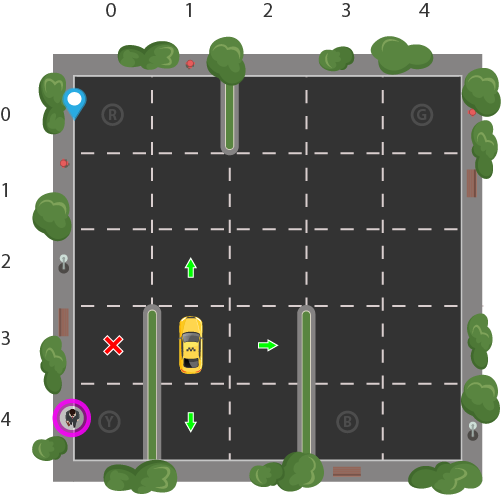
\includegraphics[scale=0.6]{rl_smart_taxi_env.png}
    \caption{Bãi tập.}
    \label{fig:training_area}
\end{figure}

Để đơn giản hóa bài toán, ta có một số giả định như sau:
\begin{itemize}
    \item Chiếc taxi là phương tiện duy nhất có trên bãi tập
    \item Khu vực huấn luyện có thể được chia thành một lưới $5 \times 5$,
    cho ta tổng cộng 25 vị trí mà chiếc taxi có thể đỗ.
    Ví dụ, như ta có thể thấy trên Hình~\ref{fig:training_area},
    chiếc taxi đang nằm tại vị trí có tọa độ (3, 1);
    ngoài ra 4 vị trí R, G, Y, B có tọa độ lần lượt là
    (0,0), (0,4), (4,0), (4,3);
    vị hành khách đáng kính đang đứng tại vị trí Y
    và có mong muốn di chuyển đến vị trí R trên bãi tập.
\end{itemize}

Vậy, ta có tổng cộng $5 \times 5=25$ vị trí mà chiếc taxi có thể xuất hiện,
4 đích đến, và 5 vị trí của hành khách
(4 vị trí tại R, G, Y, B và 1 vị trí là ở trên chiếc taxi).
Tổng số trạng thái có thể có của môi trường sẽ là
$5 \times 5 \times 5 \times 4=500$ trạng thái.

\subsubsection{Hành động}
Tại mỗi thời điểm, chiếc taxi (agent của bài toán)
sẽ nằm ở 1 trong tổng 500 trạng thái,
và nó sẽ thực hiện một hành động tương ứng với trạng thái hiện có.
Hành động ở đây có thể là đón/trả khách, và di chuyển quanh bãi tập.

Không gian hành động của ta sẽ gồm:
\begin{itemize}
    \item Đi lên
    \item Đi xuống
    \item Đi sang trái
    \item Đi sang phải
    \item Đón khách
    \item Trả khách
\end{itemize}

Để ý rằng, tại một số trạng thái ta không thể thực hiện
một vài hành động nhất định.
Ví dụ như khi chiếc taxi ở vị trí mép tường bên trái,
nó không thể thực hiện hành động đi sang trái;
ta có thể giải quyết vấn đề này bằng việc phạt chiếc taxi
khi rơi vào tình huống đó (tình huống bị "đâm" và tường)
và giữ nguyên vị trí hiện tại của nó.

\subsection{Giải quyết bài toán}
Giải pháp được sử dụng để giải quyết bài toán này
sẽ là giải thuật Q-Learning.
Môi trường của bài toán sẽ được mô phỏng nhờ vào sự trợ giúp
của thư viện Gym được cung cấp bởi OpenAI.

Chiếc taxi sẽ được huấn luyện trong 100000 episode
thông qua việc tương tác với môi trường.
Một vài kết quả được minh họa như trong Hình~\ref{fig:training_episode_step},
\ref{fig:training_episode_penalty} và \ref{fig:training_episode_reward}.

\begin{figure}[H]
    \centering
    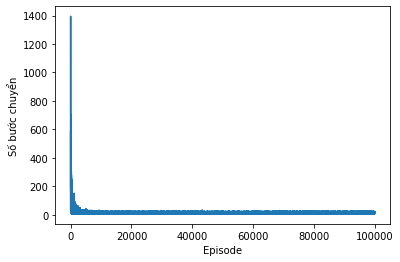
\includegraphics[scale=0.7]{training_episode_step.png}
    \caption{Số bước chuyển chiếc taxi thực hiện tại mỗi episode.}
    \label{fig:training_episode_step}
\end{figure}
\begin{figure}[H]
    \centering
    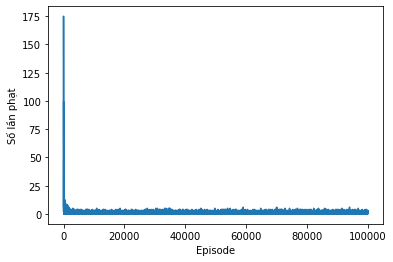
\includegraphics[scale=0.7]{training_episode_penalty.png}
    \caption{Số lần chiếc taxi đón/trả khách sai vị trí tại mỗi episode.}
    \label{fig:training_episode_penalty}
\end{figure}
\begin{figure}[H]
    \centering
    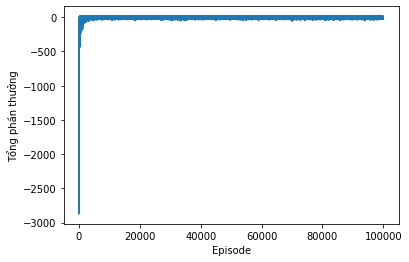
\includegraphics[scale=0.7]{training_episode_reward.png}
    \caption{Số phần thưởng chiếc taxi nhận được tại mỗi episode.}
    \label{fig:training_episode_reward}
\end{figure}

Kết quả chạy của bài toán với 1000 episode
sau quá trình huấn luyện được minh họa như trong Hình~\ref{fig:prediction_results}

\begin{figure}[H]
    \centering
    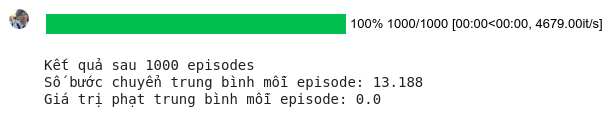
\includegraphics[scale=0.7]{prediction_results.png}
    \caption{Kết quả chạy với 1000 episode.}
    \label{fig:prediction_results}
\end{figure}

Có thể thấy chiếc taxi đã được huấn luyện khá tốt,
không mắc bất cứ sai lầm nào trong việc đón/trả khách
và thực hiện việc chọn đường đi khá "thông minh".


\section{Bài toán cân bằng con lắc ngược}



\chapter{Kết luận}
\label{ch:conc}



\backmatter

% \appendix
% \include{chapters/appendix}

\printbibliography[heading=bibintoc]

\end{document}